\documentclass[onecolumn, draftclsnofoot,10pt, compsoc]{IEEEtran}
\usepackage{graphicx}
\usepackage[section]{placeins}
\usepackage{url}
\usepackage{setspace}
 
%For indentItem command
\usepackage{enumitem}
\usepackage{changepage}

%For \textrightarrow
\usepackage{textcomp}
\usepackage{tgpagella}
 
%For Gantt Chart
\usepackage{xspace}
\usepackage{pgfgantt}
\usepackage{subcaption}
 
\usepackage{alltt}                                           
\usepackage{float}
\usepackage{color}
\usepackage{url}

\usepackage{geometry}
\geometry{textheight=9.5in, textwidth=7in}
\setlength\parindent{0pt}

\usepackage{xspace}
\usepackage{pgfgantt}
\usepackage{subcaption}

% 1. Fill in these details
\def \CapstoneTeamName{\textbf{Insert Team Name Here} }
\def \CapstoneTeamNumber{8}
\def \GroupMemberOne{James Stallkamp}
\def \GroupMemberTwo{Jeremy Fischer}
\def \GroupMemberThree{Austin Row}
\def \CapstoneProjectName{\botname}
\def \CapstoneSponsorCompany{Autodesk}
\def \CapstoneSponsorPerson{Patti Vrobel}
\def \botname{Kora\xspace}
\def \speechToText{Wit.ai\xspace}


\newenvironment{indentItem}[1][1cm]{\begin{adjustwidth}{#1}{}}{\end{adjustwidth}}

% 2. Uncomment the appropriate line below so that the document type works
\def \DocType{		%Problem Statement
				%Requirements Document
				%Technology Review
				Design Document
				%Progress Report
				}

\newcommand{\designConcernDef}[3]{
    \subsection{#1}
        \begin{tabular}[t]{r p{6in}}
            Stakeholder(s): & #2 \\
            Concern: & #3 \\
        \end{tabular}
}
\newcommand{\designConcernRef}[2][]{
    #2 #1
}
\newcommand{\designElementDef}[4]{
    \subsubsection{#1}
    \begin{tabular}[t]{r p{6in}}
        Type: & #2 \\
        Purpose: & #3 \\
        Author: & #4 \\
    \end{tabular}
}
\newcommand{\designElementRef}[2]{
    \subsubsection{#1}
    \begin{tabular}[t]{r p{6in}}
        See #2 & \\ %#2 should be element identifier (section where it's defined or ID that can be used to find it)
    \end{tabular}
}
\newcommand{\NameSigPair}[1]{\par
\makebox[2.75in][r]{#1} \hfil 	\makebox[3.25in]{\makebox[2.25in]{\hrulefill} \hfill		\makebox[.75in]{\hrulefill}}
\par\vspace{-12pt} \textit{\tiny\noindent
\makebox[2.75in]{} \hfil		\makebox[3.25in]{\makebox[2.25in][r]{Signature} \hfill	\makebox[.75in][r]{Date}}}}
% 3. If the document is not to be signed, uncomment the RENEWcommand below
\renewcommand{\NameSigPair}[1]{#1}

%%%%%%%%%%%%%%%%%%%%%%%%%%%%%%%%%%%%%%%
\begin{document}
\begin{titlepage}
    \pagenumbering{gobble}
    \begin{singlespace}
    	
\includegraphics[height=4cm]{coe_v_spot1}
        %\hfill 
        % 4. If you have a logo, use this includegraphics command to put it on the coversheet.
        \par\vspace{.2in}
        \centering
        \scshape{
            \huge CS Capstone \DocType \par
            {\large\today}\par
            \vspace{.5in}
            \textbf{\Huge\CapstoneProjectName}\par
            \vfill
            {\large Prepared for}\par
            \Huge \CapstoneSponsorCompany\par
            \vspace{5pt}
            {\Large\NameSigPair{\CapstoneSponsorPerson}\par}
            {\large Prepared by }\par
            Group\CapstoneTeamNumber\par
            % 5. comment out the line below this one if you do not wish to name your team
            %\CapstoneTeamName\par 
            \vspace{5pt}
            {\Large
                \NameSigPair{\GroupMemberOne}\par
                \NameSigPair{\GroupMemberTwo}\par
                \NameSigPair{\GroupMemberThree}\par
            }
            \vspace{20pt}
        }
        \begin{abstract}
			This Document describes the design views and components of \botname.
			This document begins by introducing the purpose, scope, and glossary, followed by a summary of the overall project.
			Then follows a list of stakeholders and their concerns.
			The rest of this document is divided into sections where each provides a different design viewpoint.
        \end{abstract}     
    \end{singlespace}
\end{titlepage}
\newpage
\pagenumbering{arabic}
\tableofcontents
% 7. uncomment this (if applicable). Consider adding a page break.
%\listoffigures
%\listoftables
\clearpage

% 8. now you write!
\section{Document Details}
	\subsection{Date of Issue and Status}
		This document was issued December 1, 2017 and is the first draft of the design document.

	\subsection{Authorship}
		Jeremy Fischer, Austin Row, and James Stallkamp are the authors of this document and the developers of \botname.
		
	\subsection{Change History}
		\begin{table}[H]
			\centering
			\caption{Change History}
			\label{my-label}
			\begin{tabular}{|l|l|}
				\hline
				\textbf{Date}     & \textbf{Change Description}   \\ \hline
				November 30, 2017 & {First design document draft} \\ \hline
			\end{tabular}
		\end{table}

\section{Introduction}
	\subsection{Purpose}
		The purpose of this design document is to outline how \botname's workflows will be completed and connected.
		More generally, this document describes how the client's requirements will be met.
		\botname's developers will use this document as a roadmap during implementation.

	\subsection{Scope}
		This document focuses on the relationships between \botname's components and their individual processes, and how they work together to satisfy the project's requirements.
	
	
	\subsection{Summary}
		\botname will be a speech-based virtual assistant for Fusion that lets users perform any one of a subset of tasks within the product, such as saving a document or opening a menu, by verbally instructing it to perform the task.
		Workflows in Fusion that are not suited for handling by a voice interface will not be supported by \botname.
		As a stretch goal, \botname will be capable of questioning the user and using responses to predict and automatically assist with future user behavior.
		It will be a plugin that is bundled with Fusion and will be part of the product's standard download. 
		
		\botname will offer users a tool that decreases the time required to achieve their goals within Fusion by offering an interface that runs in parallel with and complements the keyboard and mouse.
		If the stretch goal is achieved, \botname will further increase productivity by learning to predict and automate specific workflows within the product.

\section{Glossary}
	\begin{table}[H]
		\centering
		\caption{Glossary}
		\label{my-label}
		\begin{tabular}{|l|l|}
			\hline
			\textbf{Term} & \textbf{Definition} \\ \hline
			\botname & The virtual assistant that is the focus of this project \\ \hline
			NLP & Natural Language Processing \\ \hline
			API & Application Programing Interface \\ \hline
			CAD & Computer Aided Design \\ \hline
			CAM & Computer Aided Manufacturing \\ \hline
            UI & User Interface \\ \hline
			Fusion & An Autodesk Cloud-based 3D CAD/CAM tool/product \\ \hline
			Task & In the context of Fusion, a function or operation that can be performed in Fusion \\ \hline
			Plugin & Software that adds specific new functionality to another piece of software \\ \hline
			User & A person that interacts with \botname or Fusion depending on the context \\ \hline
			Workflow & A sequence of related tasks \\ \hline
		\end{tabular}
	\end{table}

\section{Design Stakeholders and Concerns}
    \designConcernDef{User-Application Interface}{Client, Developers}{What interfaces will exist for users to communicate to the application and for the application to communicate to users?}
    \designConcernDef{Internal Interfaces}{Developers}{What internal interfaces will exist in the software system?}
    \designConcernDef{Component Interactions}{Developers}{Which components of the software system will interact?}
    \designConcernDef{Component Interaction Responsibilities}{Developers}{What are the responsibilities of each component of the software system in the context of interactions?}
	\designConcernDef{Architecture}{Developers}{How is the system structured?}
	\designConcernDef{System States}{Developers}{What are the possible states the system can be in?}
	\designConcernDef{State Activities}{Developers}{What activity takes place in each state?}
	\designConcernDef{State Transitions}{Developers}{When does the system transition from one state to another?}
	\designConcernDef{Log Files}{Developers}{Where will user-\botname interactions be stored?}
	\designConcernDef{Log File Content}{Developers}{What will be stored in the user-\botname log files?}
	\designConcernDef{Log File Access}{Developers}{How will \botname interact with the storage system?}
	
	
%%%%%%%%%%%%%%%%%%%%%%%%%%%%%%%%%%%%%%%%%%%%%%%%%%%%%%%%%%%%%%%%%%%%%%%%%%%%%%%%%%%%%%%%%%%%%%%%%%%%%%%%%%% 
%                                           ***NOTES***
%
% Addressed Design Concerns:
%    1) Should specify by ID each of the concerns from the "Design Stakeholders and Concerns"
%       that are being addressed or discussed in that particular viewpoint.
%
% Design Elements: 
%    1) If element is not previously defined in other viewpoint, then offer definition. 
%       Otherwise reference definition in other viewpoint (e.g. "See 4.5.2")
%
% Design Rationale:
%    1) There won't be a single section for design rationale. As per the IEEE standards doc,
%       the design rationale should be justification for decisions made in the desing and
%       it doesn't need a dedicated section. Just make sure to include justification for 
%       why we chose to do something in a certain way (e.g. "Use of the Mediator design pattern
%       allows the application to...")
%%%%%%%%%%%%%%%%%%%%%%%%%%%%%%%%%%%%%%%%%%%%%%%%%%%%%%%%%%%%%%%%%%%%%%%%%%%%%%%%%%%%%%%%%%%%%%%%%%%%%%%%%%% 
\section{Design Viewpoint: Composition}
    \subsection{Addressed Design Concerns}
        \begin{itemize}
            \item \designConcernRef[4.4]{Component Interaction Responsibilities}
        \end{itemize}

    \subsection{Design Elements} 
        \designElementDef{Master Module}
                         {Module}
                         {Manages what state \botname is in and executes other modules.}
                         {James Stallkamp}
        \designElementDef{User Interface Module}
                         {Module}
                         {Provides input to \botname and expresses the state of \botname to the user.}
                         {James Stallkamp}
        \designElementDef{Speech-To-Intent Module}
                         {Module}
                         {Anaylzes speech input and produces a intent object in JSON format.}
                         {James Stallkamp}
        \designElementDef{Logger Module}
                         {Module}
                         {Stores runtime and contextual information to be used for training \botname.}
                         {James Stallkamp}
        \designElementDef{Fusion API Module}
                         {Module}
                         {Translates intent into Fusion API commands and executes them.}
                         {James Stallkamp}
        \designElementDef{Voice Synthesizer Module}
                         {Module}
                         {Synthesizes an audio output from a given text input.}
                         {James Stallkamp}
        \designElementDef{Action Prediction Module}
                         {Module}
                         {Trains \botname to become a more powerful assistant.}
                         {James Stallkamp}
						 
    \subsection{Design View: Modules}
		\botname is composed of seven primary modules.
		\subsubsection{Master Module}
			\begin{indentItem}
				The Master module, this module is responsible for coordinating all other modules.
				The master module will contain definitions for functions needed to process data objects, other modules will inherit this from master.
			\end{indentItem}
		\subsubsection{User Interface}
			\begin{indentItem}
				The User interface is the module responsible for all interaction with the user.
				This module will collect input and communicate it to the master module as well output regular feedback to the user.
			\end{indentItem}
		\subsubsection{Speed-To-Intent Module}
			\begin{indentItem}
				The speech-to-intent module will take in audio input and output a JSON object containing information on the spoken input.
				This intent module will construct the JSON object and return it to master.
			\end{indentItem}
		\subsubsection{Logger Module}
			\begin{indentItem}
				The Logger module will initialize a persist able data object containing runtime information from \botname.
				Data logged will be used to help train and improve \botname.
			\end{indentItem}
		\subsubsection{Fusion API Module}
			\begin{indentItem}
				The next module is the Fusion API module, this module will handle executing Fusion commands.
				The Fusion module will parse information from the JSON intent object to construct and execute a Fusion command.
			\end{indentItem}
		\subsubsection{Voice Synthesizer Module}
			\begin{indentItem}
				In order for \botname to speak to the user it will need a voice synthesizer module.
				This module will receive text input and produce an audio output that can be played to the user.
			\end{indentItem}		
		\subsubsection{Action Prediction Module}
			\begin{indentItem}
				The Action Prediction module is responsible for training \botname to recognize patterns and improve functionality.
			\end{indentItem}
		
\section{Design Viewpoint: Information}
	\subsection{Addressed Design Concerns}
		\begin{itemize}
			\item \designConcernRef[4.9]{Log Files}
			\item \designConcernRef[4.10]{Log File Content}
			\item \designConcernRef[4.11]{Log File Access}
		\end{itemize}


	\subsection{Design Elements}
		\designElementDef{MongoDB}{Database}{Database to hold the log files}{Jeremy}
		\designElementDef{JSON object}{Storage structure}{The structure the information will be stored in}{Jeremy}
		\designElementDef{HTTP calls}{Access mechanism}{How the data will be posted and accessed}{Jeremy}
	
	\subsection{Design View: Contents}
		The contents of the data will be:
		\begin{itemize}
			\item the intent generated by the Speech-to-Intent module
			\item the context generated by the Speech-to-Intent module such as quantities
			\item whether the user's request was successfully processed
			\item the posting date
			\item the posting time
			\item the user identification
		\end{itemize}
	
	\subsection{Design View: Access}
		The data will be posted and accessed via HTTP calls to the database.
	
	\subsection{Design View: Structure}
		The data will be stored in a MongoDB database.
		Each entry in the database will resemble the JSON object that is returned from the Speech-to-Intent module driver function.
		
		

\section{Design Viewpoint: Patterns}
    \subsection{Addressed Design Concerns}
        \begin{itemize}
            \item \designConcernRef[4.5]{Architecture}
        \end{itemize}

    \subsection{Design Elements}
		\designElementDef{Mediator Design Framework}
						 {System Architecture}
						 {\botname has a simple mediator that coordinates all interactions between all other components.}
						 {James Stallkamp}
		\designElementDef{Worker Module}
						 {Module}
						 {An inheritable module providing basic functionality to interact with the Master module.}
						 {James Stallkamp}				 
    \subsection{Design View: }
		\botname is structured according to a mediator design pattern. 
		\botname will have a Master module that coordinates interactions between itself and all other modules.
		The Master module controls Kora's flow and ensures that the correct data gets to the correct module.


\section{Design Viewpoint: Interfaces}
    \subsection{Addressed Design Concerns}
        \begin{itemize}
            \item \designConcernRef[4.1]{User-Application Interface}
            \item \designConcernRef[4.2]{Internal Interfaces}
        \end{itemize}

    \subsection{Design Elements}
        \designElementDef{UI Module Interface}{Internal Interface}{Defines rules governing interactions with the UI module.}{Austin Row}
        \designElementDef{Speech-to-Intent Module Interface}{Internal Interface}{Defines rules governing interactions with the Speech-to-Intent module.}{Austin Row}
        \designElementDef{Logging Module Interface}{Internal Interface}{Defines rules governing interactions with the Logging module.}{Austin Row}
        \designElementDef{Text-to-Speech Module Interface}{Internal Interface}{Defines rules governing interactions with the Text-to-Speech module.}{Austin Row}
        \designElementDef{Fusion Module Interface}{Internal Interface}{Defines rules governing interactions with the Fusion module.}{Austin Row}
        \designElementDef{Action Prediction Module Interface}{Internal Interface}{Defines rules governing interactions with the Action Prediction module.}{Austin Row}
        \designElementDef{Global Data Store Interface}{Internal Interface}{Defines rules governing interactions with the Global Data Store.}{Austin Row}
    \subsection{Design View: Module Interfaces}
        The interfaces to each module are driven by a single method that takes a JSON object as an argument and returns a JSON object back to the caller.
        Both the JSON object passed to the function and that which is returned contain the same two keys with values that are specific to each module and to whether it is an argument to the driver method or is a return value.
        One of the required keys is "dataIDs" which maps to an object containing key-value pairs where the key is a name specific to the target module and the value is an ID used by the global data store to identify some stored data entity.
        The second required key is "values" which maps to an object containing key-value pairs where each key is a name specific to the target module and the value is some piece of data that is to be used in the target module.
        \\[0.1in]
        For JSON that is passed as an argument to the driver method, the data IDs map to data that is stored in the global data store that is needed by the module to perform its specific functionality. 
        Also for this JSON, the "values" key-value pairs are parameters that the target module uses in to accomplish its specific responsibilities.
        For returned JSON, the data IDs map to data that was stored in the global data store by the target module during the execution of its responsibilities.
        Also for returned JSON, the "values" key-value pairs are return values that are used by modules later in the application logic flow.
        The following interface definitions describe which key-value pairs are defined for each module. 
        \\[0.1in]
        The INPUT section defines the expected format of the JSON that is passed to the module's driver function.
        The OUTPUT section defines the expected format of the JSON that is returned from the module's driver function.
        \subsubsection{UI Module Interface}
            \begin{tabular}[t]{r l p{4.5in}}
                INPUT: \{ & & \\
                & dataIDs: \{ & \\
                & & voiceResponseAudioFile: $<$dataStoreID or empty$>$ \\
                & \} & \\
                & values: \{ & \\
                & & UIActionCode: $<$number encoding what should be communicated to user through the UI$>$ \\
                & \} & \\
                \} & & \\
                OUTPUT: \{ & & \\
                & dataIDs: \{ \} & \\
                & values: \{ & \\
                & & errorOccurred: $<$0 if no errors else 1$>$ \\
                & \} & \\
                \} & & \\
            \end{tabular}

        \subsubsection{Speech-to-Intent Module Interface}
            \begin{tabular}[t]{r l p{4.5in}}
                INPUT: \{ & & \\
                & dataIDs: \{ & \\
                & & userSpeechAudioFile: $<$dataStoreID$>$ \\
                & \} & \\
                & values: \{ \} & \\
                \} & & \\
                OUTPUT: \{ & & \\
                & dataIDs: \{ & \\
                & \} & \\
                & values: \{ & \\
                & & errorOccurred: $<$0 if no errors else 1$>$ \\
                & & userCommandIntent: $<$intent JSON from Wit.ai API$>$ \\
                & \} & \\
                \} & & \\
            \end{tabular}

        \subsubsection{Speech-to-Intent Module Interface}
            \begin{tabular}[t]{r l p{4.5in}}
                INPUT: \{ & & \\
                & dataIDs: \{ & \\
                & & userSpeechAudioFile: $<$dataStoreID$>$ \\
                & \} & \\
                & values: \{ \} & \\
                \} & & \\
                OUTPUT: \{ & & \\
                & dataIDs: \{ \} & \\
                & values: \{ & \\
                & & errorOccurred: $<$0 if no errors else 1$>$ \\
                & & userCommandIntent: $<$intent JSON from Wit.ai API$>$ \\
                & \} & \\
                \} & & \\
            \end{tabular}

        \subsubsection{Logging Module Interface}
            \begin{tabular}[t]{r l p{4.5in}}
                INPUT: \{ & & \\
                & dataIDs: \{ \} & \\
                & values: \{ & \\
                & & logMessage: $<$message$>$ \\
                & & messageType: $<$error or warning or info$>$ \\
                & \} & \\
                \} & & \\
                OUTPUT: \{ & & \\
                & dataIDs: \{ \} & \\
                & values: \{ & \\
                & & errorOccurred: $<$0 if no errors else 1$>$ \\
                & \} & \\
                \} & & \\
            \end{tabular}

         \subsubsection{Text-to-Speech Module Interface}
            \begin{tabular}[t]{r l p{4.5in}}
                INPUT: \{ & & \\
                & dataIDs: \{ \} & \\
                & values: \{ & \\
                & & text: $<$text to be transcribed to speech$>$ \\
                & \} & \\
                \} & & \\
                OUTPUT: \{ & & \\
                & dataIDs: \{ & \\
                & & speechAudioFile: $<$dataStoreID$>$ \\
                & \} & \\
                & values: \{ & \\
                & & errorOccurred: $<$0 if no errors else 1$>$ \\
                & \} & \\
                \} & & \\
            \end{tabular}

        \subsubsection{Fusion Module Interface}
            \begin{tabular}[t]{r l p{4.5in}}
                INPUT: \{ & & \\
                & dataIDs: \{ \} & \\
                & values: \{ & \\
                & & userCommandIntent: $<$intent JSON from Wit.ai API$>$ \\
                & \} & \\
                \} & & \\
                OUTPUT: \{ & & \\
                & dataIDs: \{ & \\
                & \} & \\
                & values: \{ & \\
                & & errorOccurred: $<$0 if no errors else 1$>$ \\
                & \} & \\
                \} & & \\
            \end{tabular}

        \subsubsection{Action Prediction Module Interface}
            \begin{tabular}[t]{r l p{4.5in}}
                INPUT: \{ & & \\
                & dataIDs: \{ & \\
                & & userSpeechAudioFile: $<$dataStoreID$>$ \\
                & \} & \\
                & values: \{ & \\
                & & get: $<$0 if not trying to get prediction for next user command else 1$>$ \\
                & & userCommandIntent: $<$intent JSON from Wit.ai API$>$ \\
                & \} & \\
                \} & & \\
                OUTPUT: \{ & & \\
                & dataIDs: \{ \} & \\
                & values: \{ & \\
                & & errorOccurred: $<$0 if no errors else 1$>$ \\
                & & prediction: $<$empty if get=0 in input else user prediction in same format as intent data from Wit.ai API$>$ \\
                & \} & \\
                \} & & \\
            \end{tabular}

    \subsection{Design View: Data Store Interface}
        The global data store has the following methods: \\
        \begin{tabular}[t]{r p{6in}}
            Name: & Get \\
            Parameters: & dataID: The unique identifier for the data being retrieved.\\
            Return Value: & The data associated with dataID.\\
            Description: & Returns the data associated with the dataID parameter in the data store. \\
            & \\
            Name: & Store \\
            Parameters: & data: any kind of data \\
            Return Value: & The ID generated for and associated with data.\\
            Description: & Generates a unique ID and stores data associated with the ID then returns the generated. \\
            & \\
            Name: & Remove \\
            Parameters: & dataID: The unique identifier for the data being removed.\\
            Return Value: & 0 if data was not found, 1 if data was found and deleted, 2 if data was found but not successfully removed. \\
            Description: & Removes the data associated with the dataID parameter in the data store. \\
        \end{tabular}

    \subsection{Design View: User Interface}
        Placeholder

\section{Design Viewpoint: Interactions}
    \subsection{Addressed Design Concerns}
        \begin{itemize}
            \item \designConcernRef[4.3]{Component Interactions}
            \item \designConcernRef[4.4]{Component Interaction Responsibilities}
        \end{itemize}

    \subsection{Design Elements}


    \subsection{Design View: }


\section{Design Viewpoint: State Dynamics}
	\subsection{Addressed Design Concerns}
		\begin{itemize}
			\item \designConcernRef[4.6]{System States}
			\item \designConcernRef[4.7]{State Activities}
			\item \designConcernRef[4.8]{State Transitions}
		\end{itemize}
		
	\subsection{Design Elements}
		\designElementDef{Idle Listen}{State}{Kora is waiting for a wake action to take place}{Jeremy}
		\designElementDef{Active Listen}{State}{Kora begins listening to the user}{Jeremy}
		\designElementDef{Process Speech}{State}{Kora is deriving intent from the user's verbal request}{Jeremy}
		\designElementDef{Endpoint Mapping}{State}{Kora is discerning which API endpoint to call}{Jeremy}
		\designElementDef{Fusion Action}{State}{Kora makes the Fusion API call}{Jeremy}
		\designElementDef{UI Feedback}{State}{Kora is verbalizing the state of the latest request to the user}{Jeremy}
		\designElementDef{Error}{State}{Kora is in a state of error}{Jeremy}
	
	
	\subsection{Design View:  States} 
		\subsubsection{State Diagram}
			\begin{figure}[H]
				\includegraphics[width=1\textwidth, height=.35\textheight]{stateDynamics.eps}
				\centering
				\caption{The possible states \botname can be in, as well as the states the system can transfer to from within a given state.}
				\label{fig::stateD}
			\end{figure}
	
	\subsection{Design View: State Activity}
		\subsubsection{Idle Listen}
			\begin{indentItem}
				The Speech-to-Intent module is being streamed audio, but does not do anything with it until it hears the wake word or is signaled to via a wake action such as a button press.
				In this state the system is simply awaiting for the user to signal it to begin listening.
			\end{indentItem}
	
	\subsubsection{Active Listen}
		\begin{indentItem}
			The system tells the Speech-to-Intent module that it should treat the incoming audio as a request.
		\end{indentItem}
	
	\subsubsection{Process Speech}
		\begin{indentItem}
			The Speech-to-Intent module is being streamed audio and is attempting to gather intent and context from it.
		\end{indentItem}
	
	\subsubsection{Endpoint Mapping}
		\begin{indentItem}
			\botname is attempting to discern the correct Fusion API endpoint based off of the intent and context variables in the JSON received from the Speech-to-Intent module.
		\end{indentItem}
		
	\subsubsection{Fusion Action}
		\begin{indentItem}
			\botname is making the call to the Fusion API and then waiting for the API to return an error code.
		\end{indentItem}
	
	\subsubsection{UI Feedback}
		\begin{indentItem}
			\botname is signally feedback regarding the latest transaction to the user.
		\end{indentItem}
	
	\subsubsection{Error}
		\begin{indentItem}
			The system is in a state of failure and is clearing all system sub-states so \botname can attempt another request.
		\end{indentItem}
	
	
	\subsection{Design View: State Transitions}	
		\subsubsection{Idle Listen}
			\begin{itemize}
				\item \textit{Idle Listen \textrightarrow{}  Active Listen}
				\begin{indentItem}
					\botname moves from the Idle Listen state to the Active listen state when a wake action takes place.
				\end{indentItem}
			\end{itemize}
		
		\subsubsection{Active Listen}
		\begin{itemize}
			\item \textit{Active Listen \textrightarrow{}  Process Speech}
			\begin{indentItem}
				\botname moves from the Active Listen state to the Process Speech state when the Speech-to-Intent module does not receive speech for a half second.
			\end{indentItem}
			\item \textit{Active Listen \textrightarrow{}  Error}
			\begin{indentItem}
				\botname moves from the Active Listen state to the Error state when an internal failure occurs when \botname is in the Active Listen state.
			\end{indentItem}
		\end{itemize}
		
		\subsubsection{Process Speech}
		\begin{itemize}
			\item \textit{Process Speech \textrightarrow{} Endpoint Mapping}
			\begin{indentItem}
				\botname moves from the Process Speech state to the Endpoint Mapping state when the Speech-to-Intent module returns the JSON object holding the processed speech's intent and arguments.
			\end{indentItem}
			\item \textit{Process Speech \textrightarrow{} Error}
			\begin{indentItem}
				\botname moves from the Process Speech state to the Error state when an internal failure occurs when \botname is in the Process Speech state.
			\end{indentItem}
		\end{itemize}
		
		\subsubsection{Endpoint Mapping}
		\begin{itemize}
			\item \textit{Endpoint Mapping \textrightarrow{} Fusion Action}
			\begin{indentItem}
				\botname moves from the Endpoint Mapping state to the Fusion Action state when the Mapping module successfully maps the intent to a Fusion API command.
			\end{indentItem}
			\item \textit{Endpoint Mapping \textrightarrow{} UI Feedback}
			\begin{indentItem}
				\botname moves from the Endpoint Mapping state to the UI Feedback state when the Mapping module fails to map the intent to a Fusion API command.
			\end{indentItem}
			\item \textit{Endpoint Mapping \textrightarrow{} Error}
			\begin{indentItem}
				\botname moves from the Endpoint Mapping state to the Error state when an internal failure occurs when \botname is in the Process Speech state.
			\end{indentItem}
		\end{itemize}
		
		\subsubsection{Fusion Action}
		\begin{itemize}
			\item \textit{Fusion Action \textrightarrow{} UI Feedback}
			\begin{indentItem}
				\botname moves from the Fusion Action state to the UI Feedback state when the Fusion API returns the error code indicating whether the API call was successful or not.
			\end{indentItem}
			\item \textit{Fusion Action \textrightarrow{} Error}
			\begin{indentItem}
				\botname moves from the Fusion Action state to the Error state when an internal failure occurs when \botname is in the Fusion Action state.
			\end{indentItem}
		\end{itemize}
		
		\subsubsection{UI Feedback}
		\begin{itemize}
			\item \textit{UI Feedback \textrightarrow{} Idle Listen}
			\begin{indentItem}
				\botname moves from the UI Feedback state to the Idle Listen state after it indicates to the user the outcome of processing the request.
			\end{indentItem}
			\item \textit{UI Feedback \textrightarrow{} Error}
			\begin{indentItem}
				\botname moves from the UI Feedback state to the Error state when an internal failure occurs when \botname is in the UI Feedback state.
			\end{indentItem}
		\end{itemize}
		
		\subsubsection{Error}
		\begin{itemize}
			\item \textit{Error \textrightarrow{} Idle Listen}
			\begin{indentItem}
				\botname moves from the Error state to the UI Feedback state after it resets all internal variables to their initial state.
			\end{indentItem}
		\end{itemize}

\section{Gantt Chart}
   	\begin{figure}[H]
		\begin{center}
			%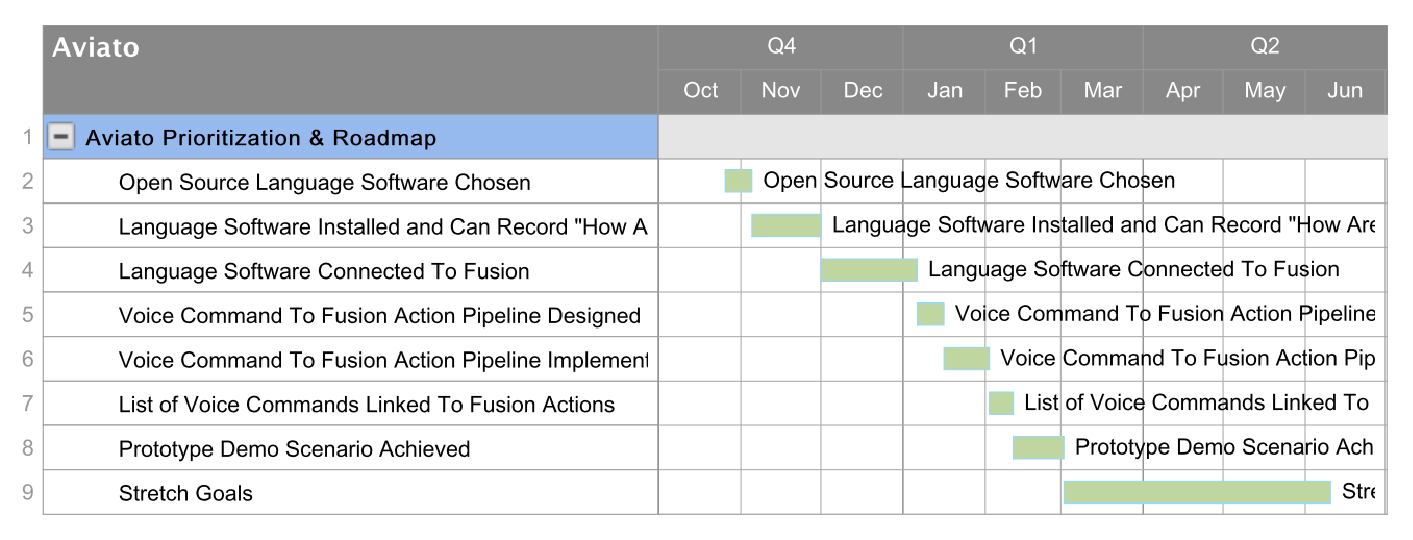
\includegraphics[width=1\textwidth]{ganttChart.eps}
			%Changed Gantt chart to be modifiable.
			\begin{ganttchart}[
				y unit title=0.4cm,
				y unit chart=0.5cm,
				vgrid,
				hgrid,
				title left shift=.05, 
				title right shift=.05, 
				title height=1, 
				group right shift=0
				]{1}{24}
				\gantttitle{Months}{24} \\
				\gantttitle{January}{4} 
				\gantttitle{February}{4} 
				\gantttitle{March}{4} 
				\gantttitle{April}{4} 
				\gantttitle{May}{4} 
				\gantttitle{June}{4} \\

				
				\ganttbar{MongoDB Creation}{1}{2} \\
				\ganttbar{Module Skeletons Creation}{1}{2} \\
				\ganttbar{Speech-to-Intent Working}{2}{3} \\
				\ganttbar{Text-to-Speech Working}{3}{3} \\
				\ganttbar{Fusion API Mapping}{2}{5} \\
				\ganttbar{Pipeline Connected}{4}{9} \\
				\ganttbar{Alpha Demo Creation}{9}{11} \\	
				\ganttbar{Performance Testing}{9}{12} \\
				\ganttbar{Train NLP Modules}{13}{20} \\
				\ganttbar{Beta Demo Creation}{17}{24} \\
				\ganttbar{Smart Assistant Stretch Goal}{15}{23} \\
				\ganttbar{Engineering Expo}{24}{24}
				
			\end{ganttchart}
			\captionsetup{justification=centering}
			\caption{\botname Development Schedule}
			\label{fig:developmentSchedule1}
		\end{center}
	\end{figure}

			
\section{Conclusion}
	This document has described \botname's development roadmap.
	This document explains the components \botname is broken up in to, and what each component is responsible for.
	Above is a Gantt chart that holds a loose development schedule which the \botname developers will abide by.
	There is a change history table at the beginning of this document which will explain any modifications made to the design described in this document.



%\bibliographystyle{IEEEtran}
%\bibliography{references.bib}



\end{document}
